\chapter{SikuliX}
	\section{Instalace}
	Po stažení balíčku započne instalace jeho spuštěním\footnote{Je potřeba instalace JRE nebo JDK 6 a~vyšší, v~linuxové distribuci balíky \emph{libopencv-core2.4, libopencv-imgproc2.4, libopencv-highgui2.4, libtesseract3} a~\emph{wmctrl} \citep{SikuliX}}. Je ukázána instalace v~Linuxu, avšak instalace ve Windows je obdobná. V~průběhu máme na výběr různé možnosti, jak chceme nástroj používat, viz obrázek \ref{Instal}. Např. zda chceme používat SikuliX-IDE a~Python nebo Ruby, jestli budeme používat jiné IDE a~Javu a~zda chceme používat OCR funkce. Zaškrtneme všechna políčka kromě \emph{Ruby (JRuby)} a~klikneme na \emph{Setup Now}. Jsme dotázáni, zda chceme balíčky stáhnout, nebo ukončit instalaci. Zvolíme \emph{Yes}. Další dotaz je na verzi Jythonu, kterou chceme použít, s~upozorněním, že může nastat problém se znaky v~kódování UTF-8. Opět zvolíme \emph{Yes}. Začne vytváření souborů a~měla by se otevřít dvě okna jako na obrázu \ref{InstalOK}, obě potvrdíme tlačítkem \emph{OK}. Pokud vše proběhne v~pořádku, vzniknou v~adresáři soubory podobné těmto\footnote{Může se lišit na různých OS} \emph{runsikulix, SetupStuff, SikuliX-1.1.0-SetupLog.txt, sikulixapi.jar, sikulix.jar}.
	\begin{figure}[ht!]
		\centering
		\caption{Instalace SikuliX}
		\label{Instal}
		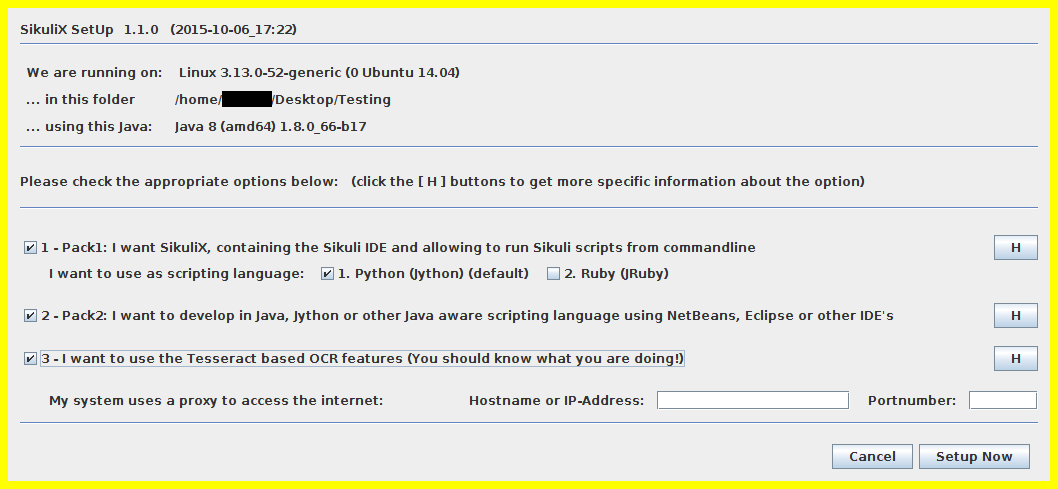
\includegraphics[width=13.5cm]{img/Instalace/Instalace.png}
	\end{figure}
	\begin{figure}[ht!]
		\centering
		\caption{Test instalace}
		\label{InstalOK}
		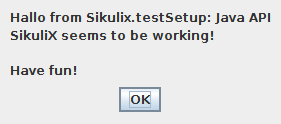
\includegraphics[width=9cm]{img/Instalace/InstalaceOK.png}\\[0.3cm]
		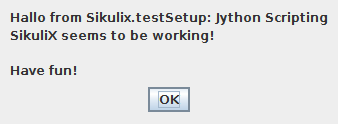
\includegraphics[width=9cm]{img/Instalace/InstalaceOK1.png}
	\end{figure}
	
	\section{Tvorba testů}
	Pro tvorbu testů pomocí SikuliX jsou nejdůležitější snímky (screenshoty) řídících prvků, které bude SikuliX hledat a~případně používat k~některým akcím. Je tedy vhodné si nejprve aplikaci spustit, vybrat příslušné prvky a~vytvořit jejich snímky. Při jejich tvorbě se doporučuje preciznost a~přesnost, neboť v~jistých situacích mohou nastat problémy, které budou zmíněny později.
	
	Pokud je vytvářený test jednoduchý a~není potřeba většího množství testů, je jednodušší vytvořit jej pomocí SikuliX-IDE. Pokud však chceme aplikaci testovat podrobněji a~psát velké množství testovacích případů, je vhodnější použít některý z~podporovaných programovacích jazyků a~využít tak jeho možnosti jako nadstavbu nad SikuliX.
	
	\section{SikuliX-IDE}
	Spustit SikuliX-IDE je možné různými způsoby \citep{SikuliX}.
	\begin{enumerate}
		\item Spuštěním souboru SikuliX.app (Mac) nebo SikuliX.exe (Windows),
		\item dvojklikem na soubor runsikulix (Linux) nebo runsikulix.cmd (Windows),
		\item z~příkazové řádky příkazem\\
		\texttt{java -jar cesta/k/sikulix.jar [volitelne parametry]}
	\end{enumerate}
	Po spuštění vypadá IDE jako na obrázku \ref{SikuliXIDE}. Jako parametry se v~metodách, ve kterých je to možné, ukazují obrázky vzorů, podle kterých se na obrazovce nástroj orientuje.
	\begin{figure}[ht!]
		\centering
		\caption{SikuliX-IDE}
		\label{SikuliXIDE}
		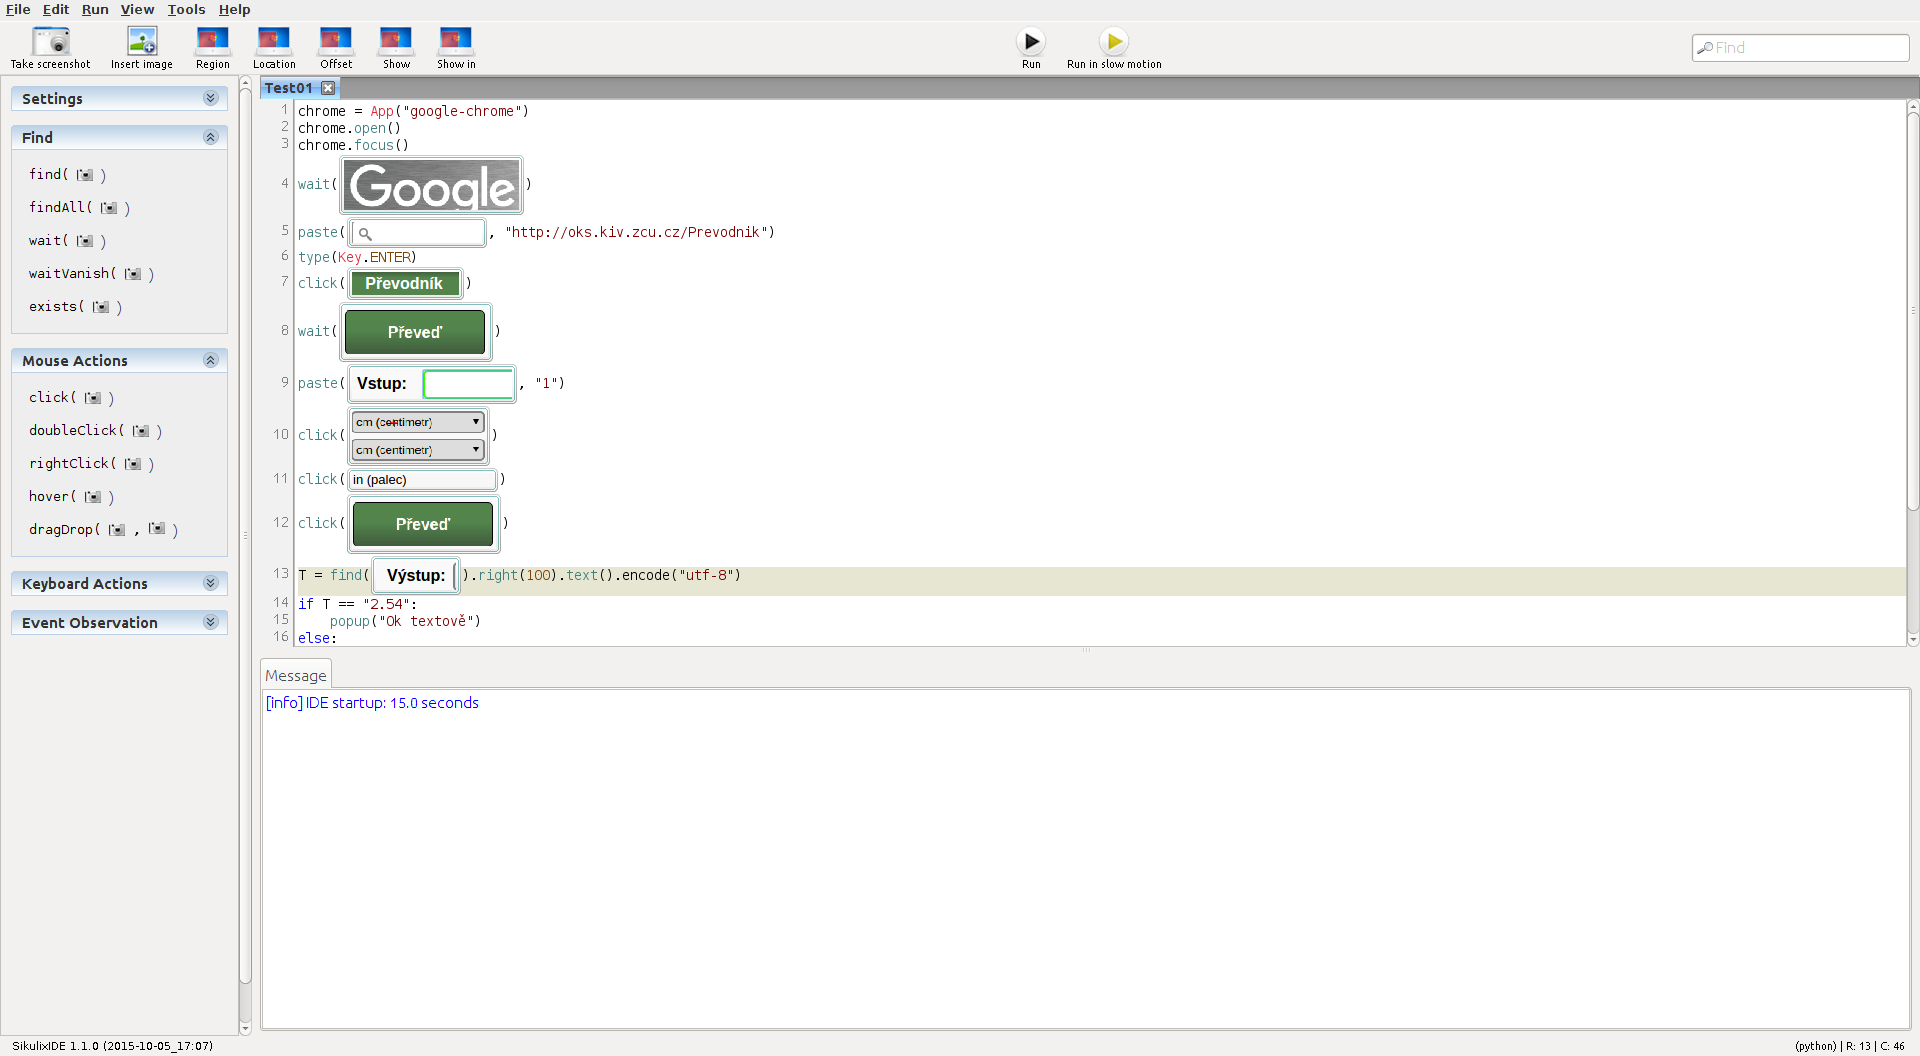
\includegraphics[width=13.5cm]{img/IDE/SikuliXIDE.png}
	\end{figure}
	
		\subsection{První skript}
		Skript se připravuje v~SikuliX-IDE, které je vidět na obrázku \ref{SikuliXIDE}. Kód, který je vidět v~\ref{PrvniSkript}, není v~IDE identický, ale cesta k~obrázku je vždy nahrazena jeho náhledem. K~tvorbě jsou v~IDE užitečné pomůcky, které se nacházejí v~levém a~v~horním panelu.
		
		Skript pracuje tak, že se otevře prohlížeč, který přejde na adresu \url{http://oks.kiv.zcu.cz/Prevodnik}. Klikne na odkaz \emph{Převodník}, do vstupního pole vloží \emph{1} a~stiskne \emph{Převeď}. Z~pole s~výsledkem přečte text a~porovná jej s~předpokládanou hodnotou \emph{2,54}. Pokud si odpovídají, objeví se dialogové okno s~potvrzením, jestliže ne, zobrazí se chybová hláška. Obdobně je tomu v~následující části, kde se pouze kontroluje existence obrázku.
		
			\begin{lstpython}{caption={První skript}, label={PrvniSkript}}
prohlizec = App("google-chrome")
prohlizec.open()	#otevre aplikaci definovanou
				#vyse
prohlizec.focus()	#vybere do popredi jeji okno
#ceka, dokud na obrazovce nenajde obrazek
wait("obr1.png")
#najde na obrazovce obrazek a vlozi do neho text
paste("obr2.png", "http://oks.kiv.zcu.cz/Prevodnik")
type(Key.ENTER)	#simuluje stisk klavesy ENTER
#najde na obrazovce obrazek a klikne na nej
click("obr3.png")
wait("obr4.png")
paste("obr5.png", "1")
#klikne o 27px vyse a 18px vlevo od nalezeneho
#obrazku
click(Pattern("obr6.png").targetOffset(-27,-18))
click("obr7.png")
click("obr4.png")
#precte text z casti, ktera je 100px vpravo od
#nalezeneho obrazku
T = find("obr8.png").right(100).text()
if T == "2.54":
	#pokud rozpoznany text souhlasi se zadanym,
	#otevre se vyskakovaci okno
    popup("Ok textove")
else:
    popError("Chyba")    #jinak se zobrazi chybove
    			 #okno

if exists("obr9.png"):
	#pokud na obrazovce existuje obrazek, otevre
	#se vyskakovaci okno
    popup("Ok obrazove")
else:
    popError("Chyba")
prohlizec.close()    #ukonci aplikaci
		\end{lstpython}
		
	\section{Java API}
	Dále bylo zkoumáno Java API, které SikuliX poskytuje. Pro jeho použití je potřeba mít při překladu a~spuštění nastavený v~classpath \emph{sikulixapi.jar}. Toho docílíme např. tak, že použijeme v~příkazové řádce dvou příkazů\\\texttt{javac -cp sikulixapi.jar:. Test01.java}\\\texttt{java -cp sikulixapi.jar:. Test01}\\ Syntaxe, kterou SikuliX v~Java API využívá, je velmi podobná té v~SikuliX-IDE.
	
		\subsection{První test}
		První test s~použitím Java API, viz kód \ref{PrvniJavaAPI}, je téměř identický s~tím, který byl vytvořen pomocí SikuliX-IDE.
		
			\begin{lstjava}{caption={První test Java API}, label={PrvniJavaAPI}}
import org.sikuli.basics.Settings;
import org.sikuli.script.*;
import javax.swing.*;

public class Test01 {

  static Screen s;
  static App prohlizec;
  
  public static void main(String [] args) {
    Settings.OcrTextSearch = true;
    Settings.OcrTextRead = true;

    s= new Screen();
    prohlizec = new App("google-chrome");
    prohlizec.open();
    prohlizec.focus();
    
    try {
      s.wait("obr1.png");
      s.paste("obr2.png");
      s.type(Key.ENTER);
      s.click("obr3.png");
      s.wait("obr4.png");
      s.paste("obr5.png", "1");
      s.click(new Pattern("obr6.png").targetOffset(
        -27,-18));
      s.click("obr7.png");
      s.click("obr4.png");
      String t = s.find("obr8.png").right(
        100).text();
      if (Double.parseDouble(t) == 2.54) {
        JOptionPane.showMessageDialog(null, "Ok" +
          " textove");
      } else {
        JOptionPane.showMessageDialog(null, "Chyba");
      }
      if (s.exists("obr9.png") != null) {
        JOptionPane.showMessageDialog(null, "Ok" +
          " obrazove");
      } else {
        JOptionPane.showMessageDialog(null, "Chyba");
      }
      prohlizec.close();
    } catch (Exception e) {
      e.printStackTrace();
    }
  }
}
			\end{lstjava}
	
		\subsection{Sofistikovanější testy}
		S~využitím knihoven \emph{JUnit} a~\emph{Log4j} (ani jedna z~těchto knihoven není pro běh SikuliX bezprostředně nutná) byly vytvořeny čtyři testy, viz kód \ref{DalsiJavaAPI}. První test skončí negativně, druhý pozitivně, třetí pozitivně a~čtvrtý negativně.